% Facultad de Ingenier\'ia, Universidad de Buenos Aires
% 75.59 Técnicas de Programación Concurrente I

\documentclass[a4paper,12pt,titlepage]{article}
\usepackage[paperwidth=180mm,paperheight=285mm,left=1.5cm,top=4cm,right=1.5cm,bottom=2cm,head=2.0cm,includefoot]{geometry}
\usepackage[spanish]{babel}
%\usepackage[latin1]{inputenc}
\usepackage[utf8]{inputenc}
\usepackage{lscape}
\usepackage{graphicx}
\usepackage{fancyhdr}
\usepackage{rotating}
%\graphicspath{{../}}

\usepackage{listingsutf8}

\title{75.59 Técnicas de Programación Concurrente I, Trabajo Práctico 1}
\author{Torres, Miguel \and Montoya, Diego \and Garay, Ignacio}

\lhead{
\includegraphics[scale=0.06]{./logo_fiuba.pdf}}
\chead{ 75.44 - Administraci\'on y control\\ de proyectos inform\'aticos I}
\rhead{}

\lfoot{Torres - Montoya - Garay}
\rfoot{\thepage}
\cfoot{$2^{do}$ Cuatrimestre 2013}

\begin{document}

\thispagestyle{empty}
% T\'itulo del documento.
\begin{center}
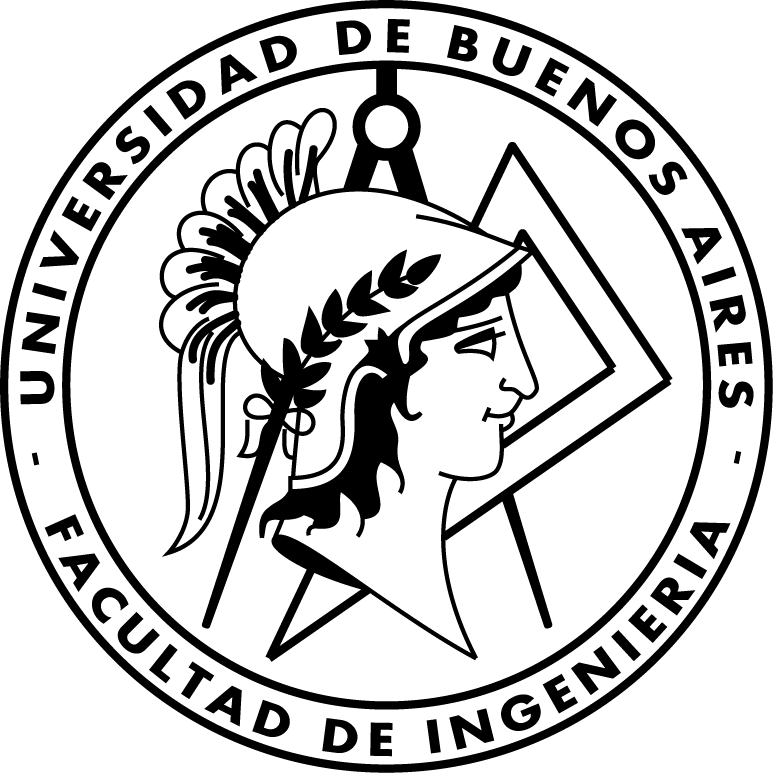
\includegraphics{./logo-fiuba.png}\\
\vspace{1cm}
\textsc{\LARGE Universidad de Buenos Aires}\\[0.3cm]
\textsc{\LARGE Facultad de Ingenier\'ia}\\[1.2cm]
\textsc{\Large 75.59 - Técnicas de Programación Concurrente I}\\[0.3cm]
\end{center}

\begin{flushright}
{\large
Montoya, Diego -- (padron)\\
Torres, Miguel -- (padron)\\
Garay, Ignacio -- 92265\\
\vspace{2cm}
$2^{do}$ cuatrimestre de 2013}
\end{flushright}

\pagestyle{fancy}
\setcounter{page}{1}
\newpage

\tableofcontents
\newpage

\footnotesize
\section{Análisis}
En el análisis del trabajo se identificaron las siguientes identidades del dominio:\\
\begin{itemize}
\item Aeropuerto
\item Avion
\item Torre
\item Control
\item Pista
\end{itemize}

El aeropuerto se podría entender como la clase que compone la torre y las pistas. El avion interactúa con el
aeropuerto, solicitando un control. Entonces el aeropuerto deriva al avión a la torre de control.
La torre de control posee varios controladores que trabajan independiente de cada uno, conectando los aviones
con las pistas. Las pistas alojan el avión hasta que el mismo ejecuta la tarea que debe, despachándolo.\\

En esta situación se puede apreciar que vamos a necesitar de algun productor de aviones
que vaya generando los aviones correspondientes. El aeropuerto, por caso, haría de consumidor.
El mismo debe derivar los aviones a la torre de control, junto con sus pistas.\\
En esta estructura vemos que se vuelve a repetir el patrón consumidor productor, donde el aeropuerto
viene a ser el productor (asignando el ingreso de aviones), mientras que el consumidor vendría a ser la torre de control.\\


\newpage
\section{Diseño}

\newpage
\section{Integración}



\end{document}


